\chapter{Hospitals in Smart Cities}
\label{abstract} 
%\usepackage{booktabs}
%\usepackage{colortbl}
%\usepackage[strings]{underscore}
%\usepackage{pdfpages}
%\usepackage{url}
\textsl{written by \\ Melanie Löbel, \\ Matriculation number 2170582
} \\ \\


\abstract
\\This chapter describes how hospitals are integrated into the "Smart City" project.
In case of an accident it is important to know which hospital is the nearest one and if it has the appropriate specialists. Also it’s important to know if the hospital or the doctor is available.
The main problem is to get those information as soon as possible because it can be essential for survival. For this purpose, each hospital must have its own ID and save the respective data such as location, existing specialists and their availability and transmitted these ones to the server. As soon as the respective hospital is contacted by the server via the corresponding topic, these information can be retrieved.
The implementation was carried out via MQTT (Message Queuing Telemetry Transport). JSON (JavaScript Object Notation) was used for simple and language independent data exchange. Python is used as programming language.

%}

\section{Introduction}
\label{sec:1}
There are a lot of working definitions for a smart city. Washburn et al. defines a smart city in this way: "The use of Smart Computing technologies to make the critical infrastructure components and services of a city - which include city administration, education, healthcare, public safety, real estate, transportation and utilities - more intelligent, interconnected and efficient." \cite{nam2011conceptualizing} In this chapter is described the healthcare in form of making a hospital search more efficient.

\section{Product overview (Context)}
\label{Hospital_Product overview}

%The research group BLABLA \cite{cheng2015building} did a similar work....using MQTT as it is shown in figure \ref{fig:1}.

By using MQTT it has to be guarantee that the hospital is registered to the server, also called the MQTT Broker \cite{zabasta2018mqtt}. Each hospital has its own stored data like location, doctors, availability and so on. The hospital must listen to the server and send the information when the responding topic is called. This happens when a client e.g. a patient is searching for a hospital or specialist. The topic that each hospital has to subscribe is '/hshl/hospitals/hospital_id'. Within this channel the data and messages should be transferred. For sending the relevant data to the server the hospital has to publish the topic '/hshl/hospitals/' too. This procedure results a context of following parts, the MQTT broker as central unit and the recipient represent as a patient and the sender consisting of three hospitals, see figure \ref{Overview environment}. 

\begin{figure}[H]
\centering
\sidecaption
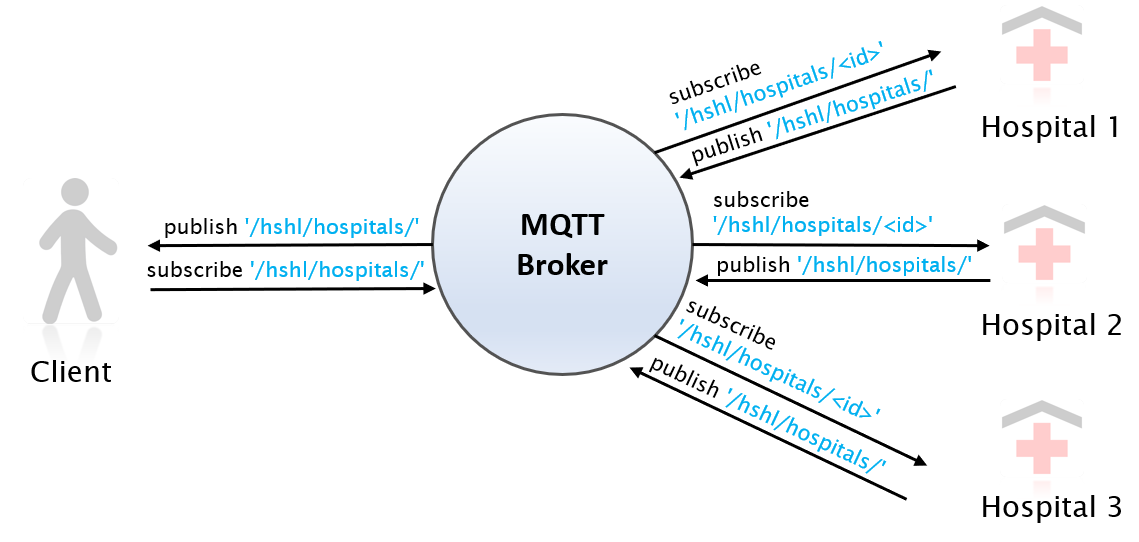
\includegraphics[scale=.375]{images/Bild1-5.png}
\caption{Overview environment and 'topic' for communication}
\label{Overview environment}
\end{figure}

%\clearpage


\section{Concept}
\label{sec:3}
In case of an accident, the person needs help as soon as possible. 
It is important not only that help arrives quickly at the accident site, 
it is also important to know where the nearest hospital is located, 
if it is available and if it has the needed specialist. For that, information such as the name of the hospital, its ID and  GPS coordinates, the number of free rooms and the specialist doctors must be stored, regularly updated and transmitted to the server.
As soon as the hospital is transferred from the server via the respective topic ''/hshl/hospitals/hospital_id'' 
these data should be displayed or sent to the server. 
\\
The patient should be able to make an appointment directly with the respective specialist e.g. in case of a light accident.
So for each doctor there must be saved information data such as specialist fields and available times.
For such function there must be realized a simple usability. The client should be able to choose functions like 'make an appointment' or 'show free rooms'. For that the concept idea is to create a menu item with select options.

%\newpage

\subsection{Requirements}
All these needed information for a hospital results in the following requirements, shown in table \ref{tab_refs}.
%\\

\begin{table}
\centering
\caption{Table of functional (FR) and non functional requirements (NFR)}
\label{tab_refs}
\setlength{\extrarowheight}{0pt}
\addtolength{\extrarowheight}{\aboverulesep}
\addtolength{\extrarowheight}{\belowrulesep}
\setlength{\aboverulesep}{0pt}
\setlength{\belowrulesep}{0pt}
\begin{tabular}{|l|l|} 
\toprule
\multicolumn{2}{|l|}{{\cellcolor[rgb]{0.753,0.753,0.753}}Requirements}                                                                                                                        \\ 
\hline
ID.                                       & Description                                                                         \\ 
\hline
\hline
\rowcolor[rgb]{0.894,0.894,0.894} 
FR 1  & The system must save user data for each hospital.                                      
\\ 
\hline
FR 1.1 & The system must save the name, the ID and the total number of free rooms.                         
\\ 
\hline
\rowcolor[rgb]{0.894,0.894,0.894} 
FR 2  & The system must save location for each hospital via GPS coordinates.               
\\ 
\hline
FR 3  & The system must save medical information about the hospital.                       
\\ 
\hline
\rowcolor[rgb]{0.894,0.894,0.894} 
FR 3.1 & The system must save the medical specialist fields.                              
\\ 
\hline
FR 3.2  & The system must save the number of doctors.                                        
\\ 
\hline
\rowcolor[rgb]{0.894,0.894,0.894} 
FR 3.3   & The system must save number of rooms within each specialist fields and their status, free or taken.         
\\ 
\hline
FR 4 & The system must check availability of doctors.                                                                
\\ 
\hline
\rowcolor[rgb]{0.894,0.894,0.894} 
FR 4.1  & The system must get a request for free appointment of a doctor.                    
\\ 
\hline
FR 4.2  & The system must check the date which was given as input.                           
\\ 
\hline
\rowcolor[rgb]{0.894,0.894,0.894} 
FR 4.2.1 & The system must check if the input date is an available date (today or in future) and if it is a weekday.    
\\ 
\hline
FR 4.3 & The system must send a message which times are available for the respective doctor.                           
\\ 
\hline
\rowcolor[rgb]{0.894,0.894,0.894} 
FR 4.4 & The system must check the time which was given as input.                           
\\ 
\hline
FR 4.4.1 & The system must check if the input time for the respective date and doctor is free.                           
\\ 
\hline
\rowcolor[rgb]{0.894,0.894,0.894} 
FR 4.5 & The system must save the appointment with patient name, date and time into the calendar from the respective doctor.  
\\ 
\hline
FR 4.6 & The system must send a message info "Accepted appointment".                                                   
\\ 
\hline
\rowcolor[rgb]{0.894,0.894,0.894} 
FR 5  & The system must check availability of rooms in a medical specialist field.                                  
\\ 
\hline
FR 5.1  & The system must get a request for availability in one medical specialist field.                             
\\ 
\hline
\rowcolor[rgb]{0.894,0.894,0.894} 
FR 5.2  & The system must send a message how many rooms are free or if there is no room available.                      
\\
\hline
FR 6  & The system must register to the server, the MQTT Broker.                      
\\
\hline
\rowcolor[rgb]{0.894,0.894,0.894} 
FR 7  & The system must listen to messages from the server.                      
\\
\hline
FR 8  & The system must send messages like the hospital info to the server.                      
\\
\hline
\hline
 

NFR 1 & Usability                                                                                                     
\\ 
\hline
\rowcolor[rgb]{0.894,0.894,0.894} 
NFR 1.1  & Menu item to choose between options like "Show free rooms", "Show specialists" and "Make an appointment".     
\\ 
\hline
NFR 2  & Efficiency                                                                                                    
\\ 
\hline
\rowcolor[rgb]{0.894,0.894,0.894} 
NFR 3 & Performance                                                                                                   
\\ 
\hline
NFR 3.1 & Guarantee that each message is received only once by the intended recipients: QoS (Quality of service) level 2                                                                                        
\\
\hline
\rowcolor[rgb]{0.894,0.894,0.894} 
NFR 3.2 & Usage of a simple and language independent data exchange format: JSON (Java Script Object Notification)                                                                                         
\\
\hline
NFR 4  & Privacy protection                                                                                             
\\ 
\hline
\rowcolor[rgb]{0.894,0.894,0.894} 
NFR 5  & Safety                                                                                                        
\\
\bottomrule
\end{tabular}
\end{table}
\newpage
\subsection{Use Case Description}
The functional requirements indicate the following use case, how the system should work with the hospital as actuator.
The hospital must be registered with the server with its own ID. In addition, the hospital has to store local information and medical data. The medical data must be updated regularly. This includes the doctors with their specialist fields and their availability regarding of free appointments. Also the availability of the hospital is needed in form of the number of free rooms. All these data should be transferred to the subscriber if the responding topic is called.
In addition the hospital should include the option to make appointments directly with the respective specialist. In case of an only light accident. For this the hospital must check the available appointments for the selected specialist when an appointment request arrives.
Depending on the availability of the appointment, the hospital should accept or reject the appointment, see figure \ref{Use_Case}.
\\

\begin{figure}[H]
\centering
\sidecaption
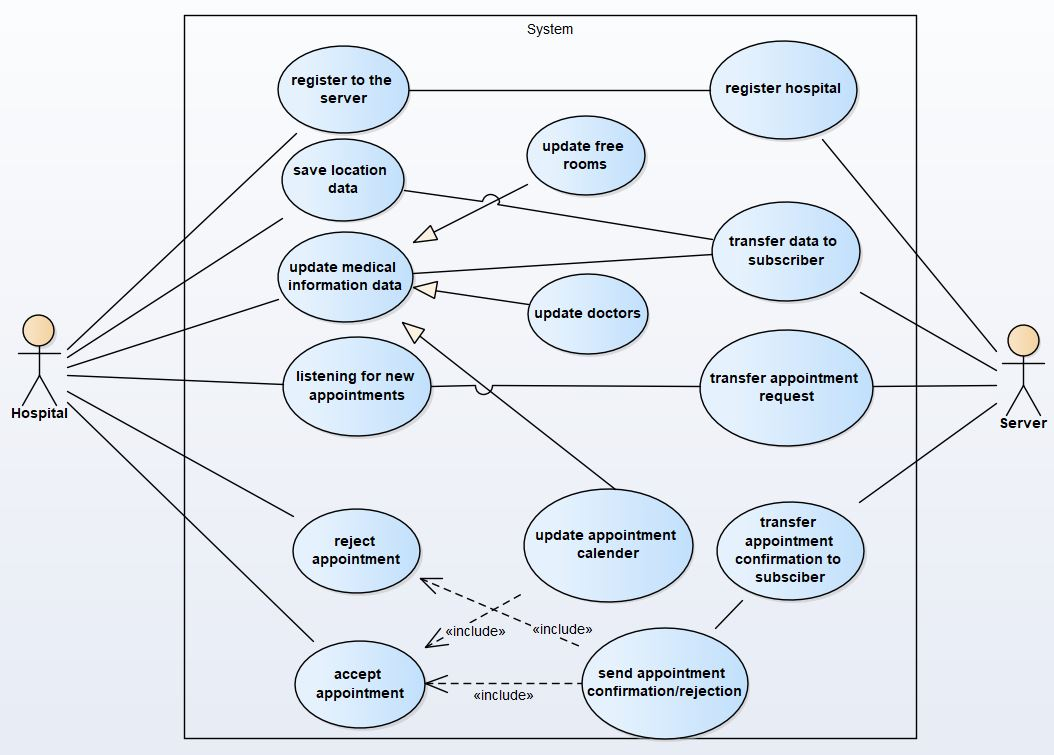
\includegraphics[scale=.425]{images/UseCase_Hospital-Search_variant-2.jpg}
\caption{Use Case Diagram}
\label{Use_Case}
\end{figure}

%For this procedure instruction it is shown in the follow class model  a concept of building up the classes following %data has to be stored in following classes

%\\ Add a picture explaining how it works (concept)
%\\ Diagrams
\\
\clearpage
\section{Implementation}
\label{sec:4}

After definition of the functional requirements and the use case, the object-oriented analysis followed to find the individual classes with attributes and necessary functions. 
A hospital has a name, an ID, a GPS location via coordinates and a number of free rooms. In addition, each hospital has several doctors. They have a title, a name, and a phone number. Each doctor is a specialist in one or more fields. In addition, every doctor is available at certain times on weekdays. That can be in the morning and/or in the afternoon. The doctors with their specialist fields, the number of free rooms and all busy appointments are to be displayed via a query. In addition, an appointment with a doctor should be able to be arranged with a date and time. Appointments are only compatible on weekdays and in the future. In case of an accident and for the search for a suitable hospital nearby, the server must have the following data: name of the hospital, the ID, the GPS location, the number of doctors and free rooms and the specialist fields of all doctors, in order to have the respective specialist depending on the type of an accident. These data has to be stored in one message which has to be transmitted to the server via JSON format. 
For the required communication to the server there should be a separate class 'Communication' implemented which contains the topic with all necessary methods for MQTT communication. So the class 'Communication' should ensure that the hospital communicates via publish and subscribe the respective topic. 
In following figure \ref{Class_diagram} the different classes with their needed attributes and methods are simply described.

\begin{figure}[H]
\centering
\sidecaption
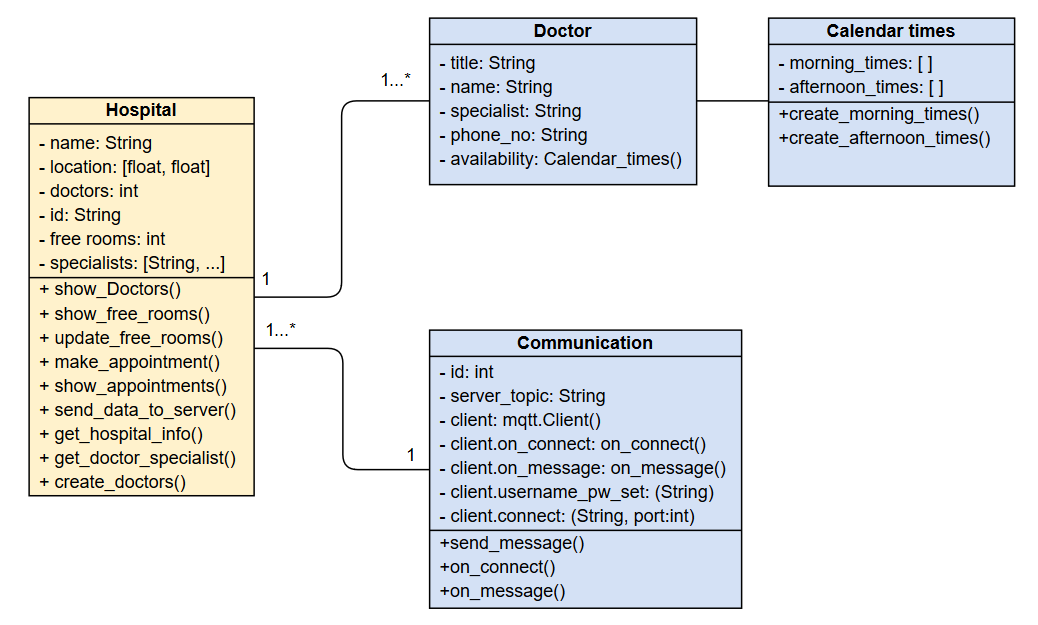
\includegraphics[scale=.425]{images/Class_model.png}
\caption{Class Diagram}
\label{Class_diagram}
\end{figure}

\\
\subsection{Classes with relation to requirements}
\subsubsection{Communication}
Important for the MQTT communication is to import the mqtt client, see figure \ref{Communication} line 1. For using the JSON data exchange (NFR 3.2) json has to be imported too. For the procedure to make an appointment with the doctor the package time has to be imported. Next to the topic '/hshl/hospitals/' the connect and message event must be also assigned. In addition the user name, the password and the broker address is needed to connect with it (FR 6). For listening to the server the method 'on_connect' is needed (FR 7). For sending a message the methods 'send_message' and 'on_message' must be included (FR 8). The hospital is only response when it is directly selected about the topic and its self.id. The relevant data will be send as a message in JSON format about the general topic '/hshl/hospitals/', see line 23 in figure \ref{Communication}.

\begin{figure}[H]
\centering
\sidecaption
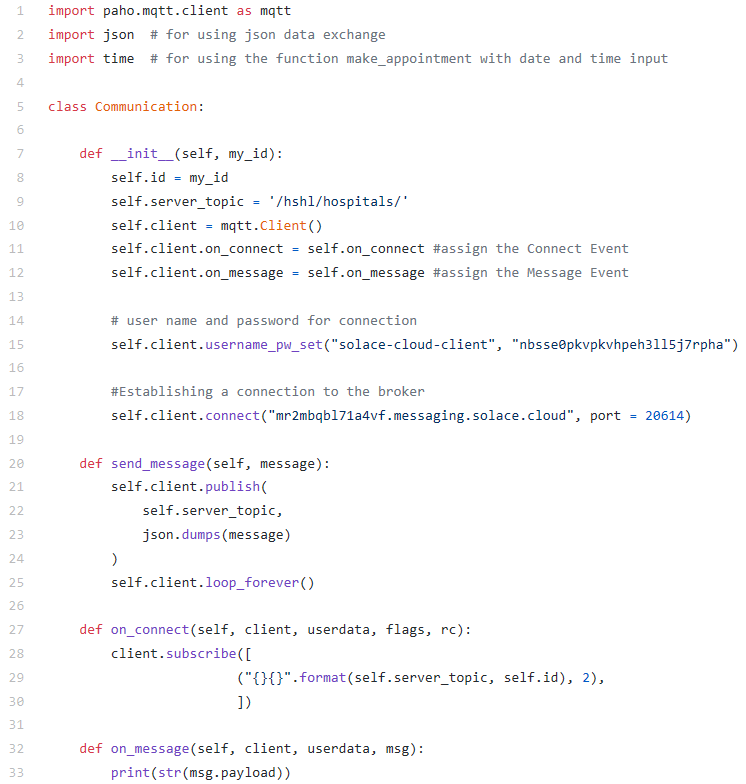
\includegraphics[scale=.53]{images/Communication.png}
\caption{Class Communication}
\label{Communication}
\end{figure}

In line 29 in figure \ref{Communication} the QoS level is set to '2' like required with NFR 3.1. It is the highest level of service in MQTT. This level guarantees that each message is received only once by the intended recipients. QoS 2 is the safest and slowest quality of service level. The guarantee is provided by at least two request/response flows (a four-part handshake) between the sender and the receiver \cite{ferguson1998quality}.

\subsubsection{Doctor and Calendar times}
In the class Doctor it's only necessary to create the constructor with the needed attributes like described in the class diagram in figure \ref{Class_diagram}. Important is that here are two methods. One method for returning the title, name and specialist field from the doctor as info string and the other method for representation or displaying it. 

\begin{figure}[H]
\centering
\sidecaption
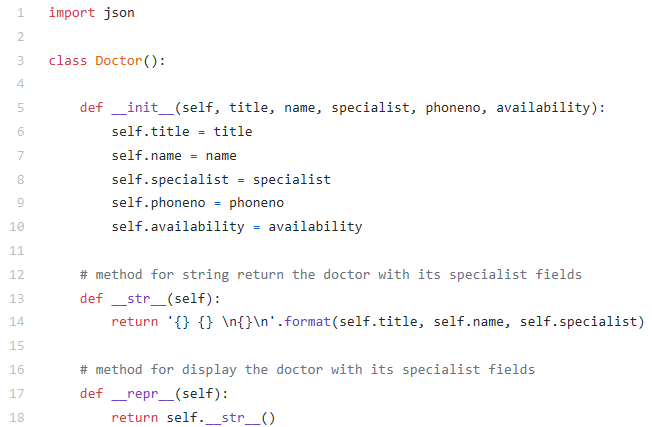
\includegraphics[scale=.65]{images/Doctor.png}
\caption{Class Doctor}
\label{Doctor}
\end{figure}

The next important class which affects the appointment making is 'Calendar times'. It contains the available times when a doctor would be available. It's separated in morning and afternoon times. Later in the hospital class a doctor can be created as a new object which has both available times in the morning and in the afternoon or only one of it. Important is here to import datetime.

%\begin{figure}[H]
%\centering
%\sidecaption
%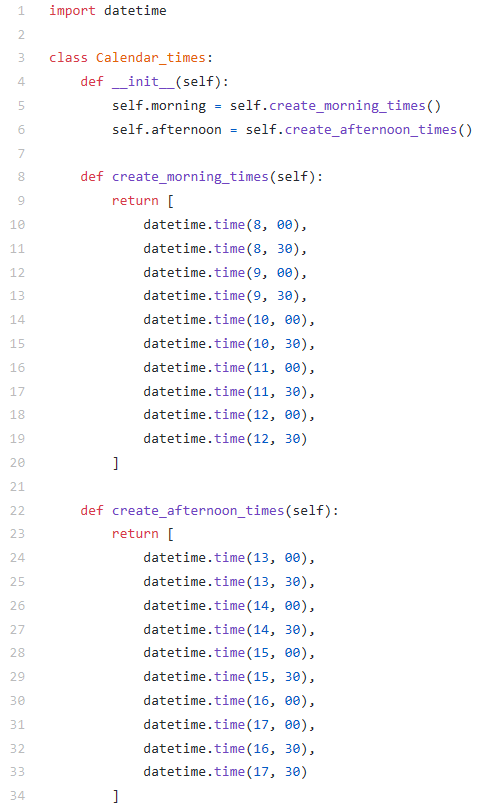
\includegraphics[scale=.65]{images/Calendar_times.png}
%\caption{Available calendar times}
%\label{Calendar_times}
%\end{figure}

\begin{figure}[t]
\begin{minipage}[t]{0.475\textwidth}
\centering
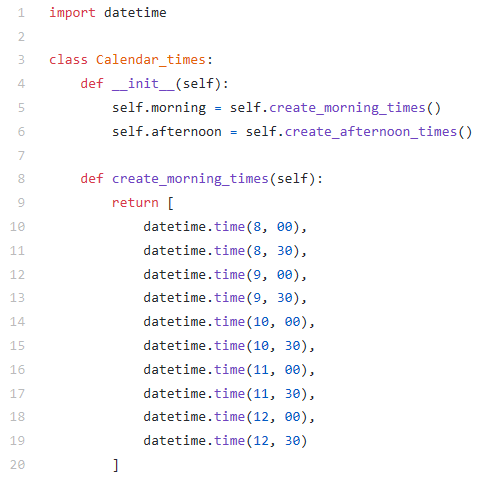
\includegraphics[scale=.65]{images/Calendar_times-1.png}
    \caption{Available calendar times}
    \label{Calendar_times}
\end{minipage}
\hfill
\begin{minipage}[t]{0.475\textwidth}
\centering
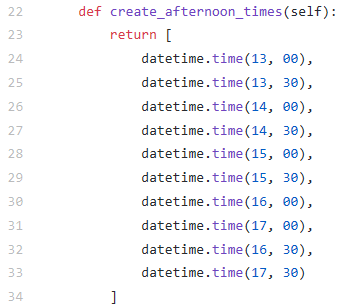
\includegraphics[scale=.65]{images/Calendar_times-2.png}
    %\caption{2}
    \label{2}
\end{minipage}
\end{figure}

\subsubsection{Hospital}
The main important class is the hospital. The other classes like Communication, Doctor and Calendar times has to be imported into the class Hospital. In addition for make an appointment also the packages datetime and calendar are needed to be imported. In figure \ref{hospital_attributes} is represented the needed attributes which are required in FR1, FR2, FR3.1, FR3.2, FR4.5.

\begin{figure}[H]
\centering
\sidecaption
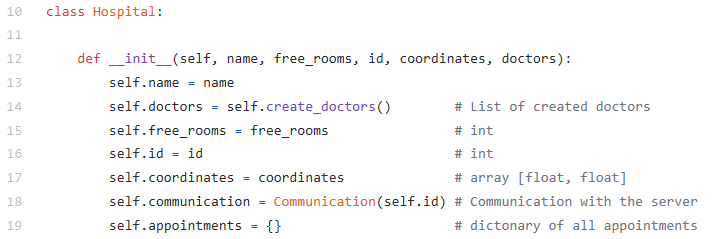
\includegraphics[scale=.65]{images/Relevant_attributes_in_the_hopital_class.png}
\caption{Needed attributes in the class Hospital}
\label{hospital_attributes}
\end{figure}


In the project 'Smart City' the main requirement is that the attributes which are shown in figure \ref{Relevant_attributes_server} in the dictionary 'hospital_info' will be send to the server. Including name and location coordinates of a hospital, the total number of doctors, the hospital ID, the total number of free rooms and the specialist fields. So the first step is to get these data and stored it into 'hospital info' as a dictionary. This structure is necessary for sending data in JSON format \cite{sporny2019json}. Also it is relevant return this hospital info so that another method have access to this info, see line 184 in figure \ref{Relevant_attributes_server}. 

\begin{figure}[H]
\centering
\sidecaption
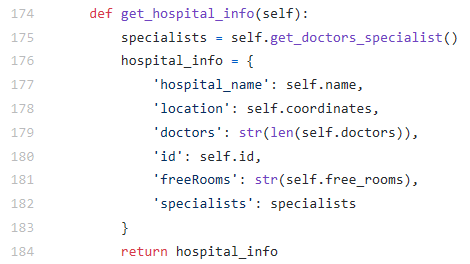
\includegraphics[scale=.65]{images/get_hospital_info.png}
\caption{Relevant attributes for the server}
\label{Relevant_attributes_server}
\end{figure}

With the variable 'message' the hospital info will be saved about the access on method self.get_hospital_info(). Afterwards this message will be send to the server with the access to the class Communication, see line 172 in figure \ref{send_hosp_info}. 


\begin{figure}[H]
\centering
\sidecaption
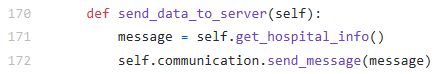
\includegraphics[scale=.7]{images/send_hospital_info.png}
\caption{Data transfer method for sending to the server}
\label{send_hosp_info}
\end{figure}

Like in introduction in subsection \ref{tab_refs} described it should be also feasible to make an appointment with a doctor itself, see requirement FR4. The activity diagram in figure \ref{Make_Appointment} shows how this requirement with its sub requirements are implemented. It's represented the single steps until the appointment is accepted. So after a date is entered it will be check if it is a weekend or if this date is in the past. For these both situation a new date has to be entered. It's realized with an if and elif condition. If both situation are not true the else condition continues and a request for a time will be send. The next step is to check if the entered time is available for this date with the respective doctor. For that all appointments has to be summarized in a dictionary.

\begin{figure}[H]
\centering
\sidecaption
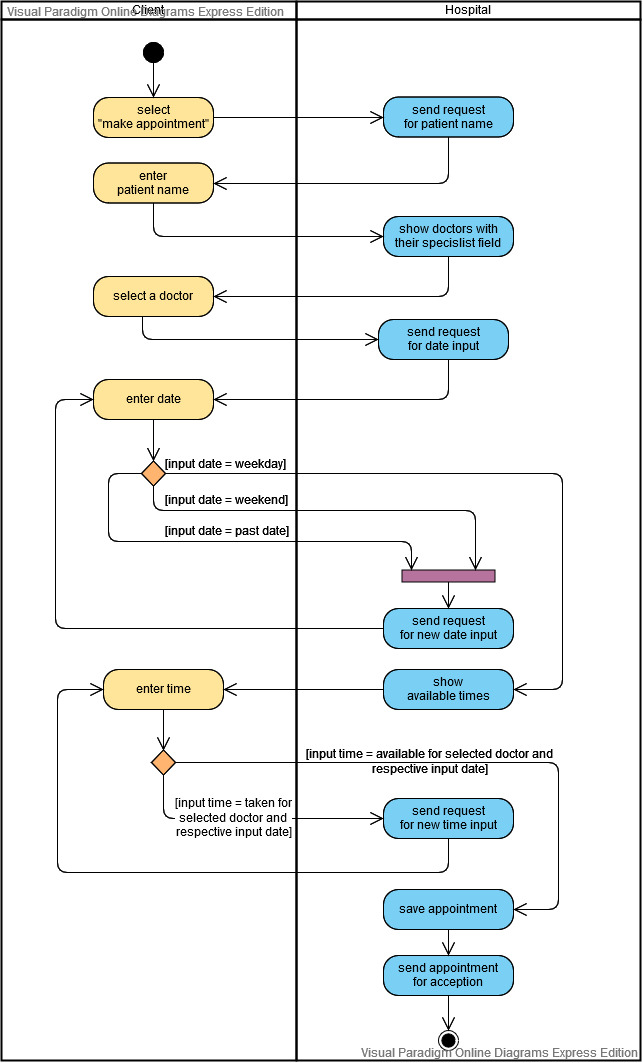
\includegraphics[scale=.55]{images/MakeAppointment.jpg}
\caption{Activity Diagram "make an appointment"}
\label{Make_Appointment}
\end{figure}

For being sure that a room is available when it's needed there will be a room reserved in condition that an appointment is accepted. An info message for this is sent and the number of rooms will be adapt. %, see cut out of the code in the hospital.py, figure \ref{Acception}.

%\begin{figure}[H]
%\centering
%\sidecaption
%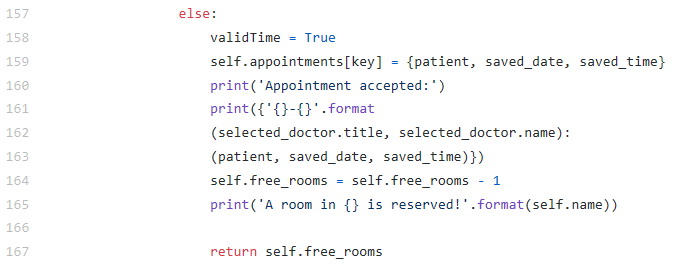
\includegraphics[scale=.65]{images/Acception.png}
%\caption{Acceptation message of an appointment with room reservation }
%\label{Acception}
%\end{figure}

\subsubsection{Usability}
To have something like an overview about the main functions the non functional requirement NFR 1.1 was to have a menu item with the possibility to choose options like 'make an appointment' or 'show free rooms'. The possible options or functions which were implemented are described in figure \ref{Options}. It shows a cut out of the class Hospital.

\begin{figure}[H]
\centering
\sidecaption
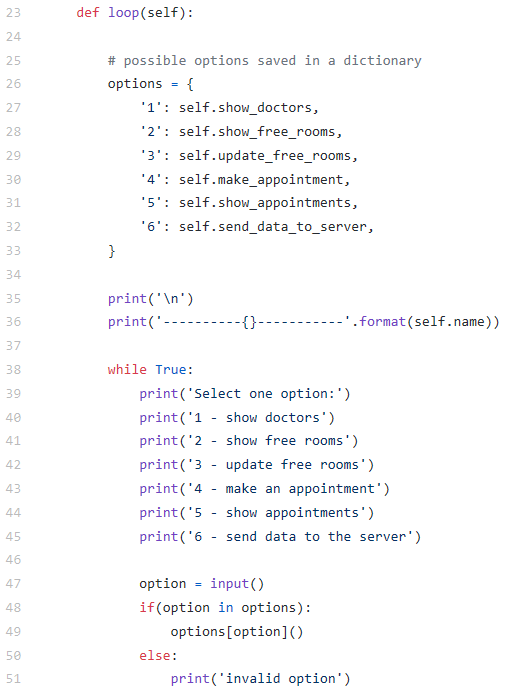
\includegraphics[scale=.65]{images/Options.png}
\caption{Implementation menu item}
\label{Options}
\end{figure}

The functions 'make an appointment' and 'send data to the server' were described in more detail in the sub sections before. the other four functions are very simply in the implementation. It contains only the output via 'print' so that the info is displayed directly. With 'update free rooms' there is the possibility to save a new number via input() of rooms.

\subsubsection{Realization of three hospitals}
Like described in the beginning of this capture in the product overview \ref{Hospital_Product overview} there should be three hospitals. To implement more than one hospital in a smart city there were implemented three additional files: main1.py, main2.py and main3.py.
Here the object Hospital from the class hopital.py is imported. Also the objects Doctor and Calendar_times are needed. So that e.g. in each main.py the respective hospital with its doctors can be initialized.

\section{Results}
\label{sec:5}
In summary the most of the requirements were implemented. This concerns the functional ones FR 1 until FR 4 and FR 6 until FR 8. The sub requirement FR 3.3 were implemented only partly. Only the total number of free rooms were considered and not for each medical specialist field. In condition to that also FR5 with the availability check for each medical specialist field is not full implemented.  But it would be possible to do this in future work with creation of medical stages in each hospital which have a number of rooms. So the code is extendable. In view of the non functional requirements the NFR 1, the usability was full filled with the different select able options. Like described NFR 3 was implemented by setting the QoS level 2 and by using JSON format. The privacy protection described in NFR 4 was already implemented e.g. in hospital.py with the method 'def __init__()'. This format defines a private method. The safety with NFR 5 isn't implemented yet. To increase the efficiency which is required in NFR 2 the function 'make_appointment' could be improved. The function could be adapted in that way that only the times for each doctor will be shown which are free at the chosen date. Currently all times from the doctor are shown. If a time is selected which is taken for the chosen date an info message is send to choose another time. This procedure can be avoid if only the valid times for the chosen date are displayed.
\\

\section{Conclusion}
\label{sec:5}
This capture showed in detail how a hospital could be implemented in the project 'Smart city'. It was given an overview about the requirements and how they were implemented into a python code including usage of MQTT and JSON data transfer. The python code is find below following link \url{https://github.com/melanieloebel/Interaktionskonzept_ITD_MelanieLoebel.git}. The hospital could be upgraded in future work. For example with an emergency room. So that in case of an hard accident this room can be reserved.

\newpage
\bibliographystyle{IEEEtran}
\bibliography{chapter3.bib}
